\section{Api-Service}

Daten werden an den API-Service im Body einer Anfrage im form-data Format übergeben.
So kann man neben den Informationen zu der Datenquelle in der gleich Anfrage auch weitere Dateien mit hochladen.
Dabei werden alle Daten als Schlüssel-Wert-Paar übertragen.
Für die DatasourceDefinition muss der Schlüssel "`datasource-definition"' verwendet werden.
Die Schlüssel der hochgeladenen Dateien sind frei wählbar.
Die Eingabe der DatasourceDefinition wird im JSON Format übertragen.
\fref{fig:datasource-definition-input} zeigt das dazugehörige Modell.

\begin{figure}
    \centering
    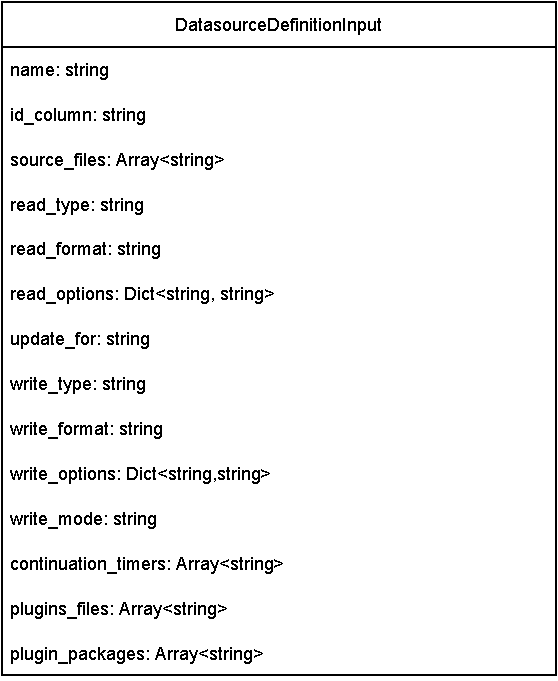
\includegraphics[width=.65\textwidth]{Grafiken/Umsetzung-Definition-Input.pdf}
    \caption{Felder Datenquellen-Eingabe}
    \label{fig:datasource-definition-input}
\end{figure}

\subsection{Hochladen von Dateien}

Für jede Datenquelle können Quell- oder Plugindateien hochgeladen werden.
Ein Eintrag in der Liste der Dateien kann entweder ein Dateiname oder der Schlüssel einer Datei sein, die in der Anfrage mitgesendet wird.
Bei der Verarbeitung der Eingabe prüft der Api-Service für jeden Eintrag der Listen, ob eine Datei mit diesem Schlüssel hochgeladen wurde.
Ist das der Fall, wird die entsprechende Datei in das HDFS hochgeladen und der Name der Datei der neuen Revision angehangen.
Wenn keine Datei in der Anfrage gefunden wurde, wird geschaut ob im HDFS eine Datei mit dem Namen existiert.
Wird eine Datei gefunden, wird der Name an die neue Revision angehangen.
Sonst wird dieser Eintrag ignoriert.
